\section{PnP}
\begin{itemize}
  \item \textbf{Got:} 2D-3D correspondences
  \item \textbf{Want:} $T, R$ between camera and world coordinate
    system.
\end{itemize}

\textbf{Solutions}
\begin{itemize}
  \item Linear hack (hw 3)\\
    $\lambda_i \begin{pmatrix} x_i \\ y_i \\ 1 \end{pmatrix} = R
    \begin{pmatrix}X_i \\ Y_i \\ Z_i \end{pmatrix} + T$\\
    Expand the matrices.
    Solve for $\lambda_i$, and get two equations per point. \alert{We
    need at least 6 points}.
  \item Non-linear optimization
  \item P3P
\end{itemize}

\subsection*{P3P}
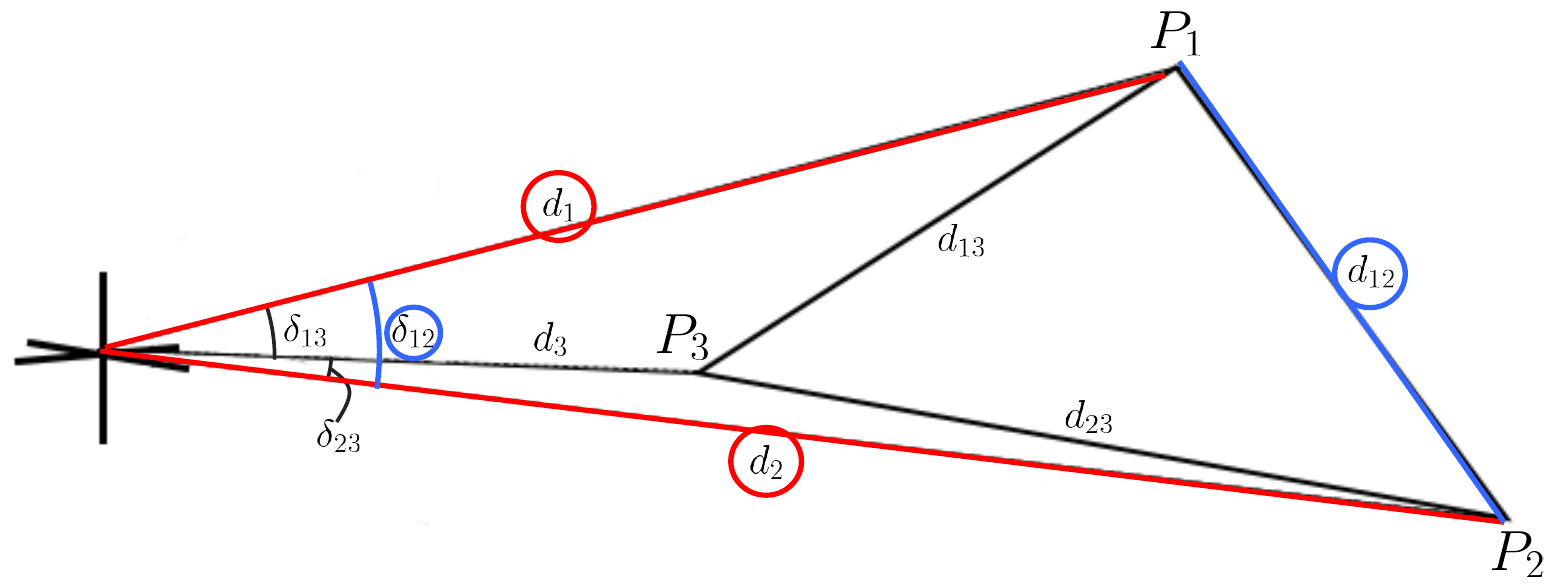
\includegraphics[width=\linewidth]{Images/P3P.png}
Simple formulation:\\
$d_i^2 + d_j^2 - 2 d_i d_j \cos(\delta_{ij}) = d_{ij}^2$\\
\alert{Use this for simple problems!}

Complex formulation: we use $d_2 = u d_1$, $d_3 = v d_1$, then:\\
$d_{13}^2 (u^2 + v^2 - 2 u v \cos(\delta_{23}) \\= 
d_{23}^2(1+v^2 - 2 v cos(\delta_{13}))$\\
$d_{12}^2 (1 + v^2 - 2v \cos(\delta_{13})) \\=
d_{13}^2 (1 + u^2 - 2u \cos(\delta_{12}))$
\begin{enumerate}
  \item Solve $u^2$ in 1.
  \item Insert $u^2$ back into 2.
  \item Solve $u$, leaving terms in $v$ and $v^2$.
  \item Insert $u$ back into 1. Quartic polynomial in $v$.
    \alert{At most 4 solutions}.
\end{enumerate}

\alert{To find the angles, we can use the dot product of the rays.}
Each pixel on the camera image denotes a direction. Using camera K matrix, you can find the vector in the camera frame. Using inner products give the angle cosines.

After solving P3P, we have to use Procrustes to find $R$ and $T$.
